\let\negmedspace\undefined
\let\negthickspace\undefined
\documentclass[journal]{IEEEtran}
\usepackage[a5paper, margin=10mm, onecolumn]{geometry}
%\usepackage{lmodern} % Ensure lmodern is loaded for pdflatex
\usepackage{tfrupee} % Include tfrupee package

\setlength{\headheight}{1cm} % Set the height of the header box
\setlength{\headsep}{0mm}     % Set the distance between the header box and the top of the text

\usepackage{gvv-book}
\usepackage{gvv}
\usepackage{cite}
\usepackage{amsmath,amssymb,amsfonts,amsthm}
\usepackage{algorithmic}
\usepackage{graphicx}
\usepackage{textcomp}
\usepackage{xcolor}
\usepackage{txfonts}
\usepackage{listings}
\usepackage{enumitem}
\usepackage{mathtools}
\usepackage{gensymb}
\usepackage{comment}
\usepackage[breaklinks=true]{hyperref}
\usepackage{tkz-euclide} 
\usepackage{listings}
% \usepackage{gvv}                                        
\def\inputGnumericTable{}                                 
\usepackage[latin1]{inputenc}                                
\usepackage{color}                                            
\usepackage{array}                                            
\usepackage{longtable}                                       
\usepackage{calc}                                             
\usepackage{multirow}                                         
\usepackage{hhline}                                           
\usepackage{ifthen}                                           
\usepackage{lscape}
\begin{document}

\bibliographystyle{IEEEtran}
\vspace{3cm}

\title{3.3.20}
\author{EE24BTECH11011-B.PRANAY KUMAR
}
 \maketitle
% \newpage
% \bigskip
{\let\newpage\relax\maketitle}

\renewcommand{\thefigure}{\theenumi}
\renewcommand{\thetable}{\theenumi}
\setlength{\intextsep}{10pt} % Space between text and floats


\numberwithin{equation}{enumi}
\numberwithin{figure}{enumi}
\renewcommand{\thetable}{\theenumi}



\textbf{Question}:\\
Draw a triangle $PQR$ in which $QR = 3$ cm, $QP - PR = 6$ cm, and $\angle PQR = 45\degree$.\\

\textbf{Solution}:\\
For triangle $PQR$ with $QR = 3$ cm, $QP - PR = 6$ cm, and $\angle PQR = 45\degree$.

From the Law of Cosines(3.1.1.1)

\begin{align}
	QP^2 &= QR^2 + PR^2 - 2 (QR) ( PR )  \cos\angle PQR 
\end{align}

Let $k$ be defined as:

\begin{align}
    k &= QP - PR
\end{align}

So, the expression for $QP$ in terms of $k$ is:

\begin{align}
	QP &= \frac{k^2 + QR^2}{2 ( \left(k - QR  \cos\angle PR\right)}
\end{align}

where $\angle PR$ is the angle opposite side $QR$.\\

 Therefore, the side lengths are approximately:
   \begin{enumerate}
       
       \item $QR = 3$ cm
       \item $PR \approx 1.67$ cm
       \item $QP \approx 7.67$ cm
   \end{enumerate}
\begin{figure}[h!]
   \centering
   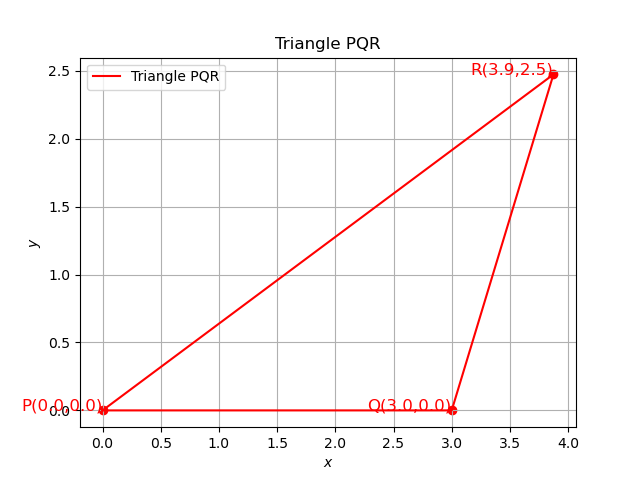
\includegraphics[width=0.7\linewidth]{figs/triangle_pqr_plot.png}
   \caption{Triangle $PQR$}
\end{figure}

\end{document}


